\documentclass[12pt]{article}
\usepackage[english]{babel}
\usepackage[utf8x]{inputenc}
\usepackage{amsmath}
\usepackage{graphicx}
\usepackage{listings}
\usepackage{booktabs}
\usepackage{float}

\begin{document}

\begin{titlepage}

\newcommand{\HRule}{\rule{\linewidth}{0.5mm}} % Defines a new command for the horizontal lines, change thickness here

\center % Center everything on the page
 
%----------------------------------------------------------------------------------------
%   HEADING SECTIONS
%----------------------------------------------------------------------------------------

\textsc{\LARGE Lebanese American University}\\[1.5cm] % Name of your university/college
\textsc{\Large CSC447: Parallel Programming for Multi-Core and Cluster}\\[0.5cm] % Major heading such as course name
\textsc{\large Course Project: A Parallel Monte Carlo Simulation for Black-Scholes Option Valuation}\\[0.5cm] % Minor heading such as course title

%----------------------------------------------------------------------------------------
%   TITLE SECTION
%----------------------------------------------------------------------------------------

\HRule \\[0.4cm]
{ \huge \bfseries Project Report}\\[0.4cm] % Title of your document
\HRule \\[1.5cm]
 
%----------------------------------------------------------------------------------------
%   AUTHOR SECTION
%----------------------------------------------------------------------------------------

\begin{minipage}{0.4\textwidth}
\begin{flushleft} \large
\emph{Author:}\\
Sabrina \textsc{Azar} % Your name
\end{flushleft}
\end{minipage}
~
\begin{minipage}{0.4\textwidth}
\begin{flushright} \large
\emph{Supervisor:} \\
Dr. Haidar \textsc{Harmanani} % Supervisor's Name
\end{flushright}
\end{minipage}\\[2cm]

% If you don't want a supervisor, uncomment the two lines below and remove the section above
%\Large \emph{Author:}\\
%John \textsc{Smith}\\[3cm] % Your name

%----------------------------------------------------------------------------------------
%   DATE SECTION
%----------------------------------------------------------------------------------------

{\large \today}\\[2cm] % Date, change the \today to a set date if you want to be precise

%----------------------------------------------------------------------------------------
%   LOGO SECTION
%----------------------------------------------------------------------------------------


\includegraphics[scale=0.5]{logo}\\[1cm] % Include a department/university logo - this will require the graphicx package
 
%----------------------------------------------------------------------------------------

\vfill % Fill the rest of the page with whitespace

\end{titlepage}


\section{Experimental Setup}

For experimental testing I first used my laptop, a Macbook Pro 2016. This works
for OpenMP and for testing if the code works or not, but is not good for
testing OpenACC because OpenACC does not support the GPU on macOS.

Therefore, I also used the computers in the computer labs at LAU for
experimenting and comparing speedups. The computers in the lab run Ubuntu 14.04
LTS, have 15.6 GiB of RAM, a Intel Xeon CPU E5-1620 v4 @ 3.50 GHz x 8 processor
and Quadro K420 for Graphics.

For editing the code, I used Visual Studio Code on my Macbook (except when I
had to use the computer labs to test OpenACC). For compiling and running the
program, I used iTerm:

\begin{lstlisting}
make clean
make all
time ./csc447.x params.txt NUMBER OF THREADS
\end{lstlisting}

For example (4 threads):

\begin{lstlisting}
make clean
make all
time ./csc447.x params.txt 4
\end{lstlisting}

\section{Experimentation: Black-Scholes Parameters}

I tried changing each line in params.txt, one by one (to test smaller and
larger values). For example, I would change the first line but keep all the
others unchanged. The only two parameters that made a difference were the fourth
parameter (gamma) and the last one (the number of trials). When gamma is very
high, the simulation is faster. The number of trials also affects the time, of
course: when the number of trials is high, the simulation takes more time.

\section{Experimentation: Number of Threads}

First, we set the number of trials to 10,000,000. Increasing the number of
threads leads to a decrease in simulation time. This shows that my
parallelization code is working correctly. When I use too many threads (more
than there are cores), I get a small speed decrease. This is normal because the
cores are then each switching between 2 tasks, instead of each focusing on one
task, so some time is lost between the switching.

\section{Speedup and performance analysis}

\begin{table}[H]
\centering
\caption{Simulation Time Comparison}
\label{my-label}
\begin{tabular}{@{}lll@{}}
\toprule
Number of threads & Sim time (OpenMP) & Sim time (OpenACC) \\ \midrule
1                 & 1.32 s            & 0.72 s             \\
2                 & 0.83 s            & 0.48 s             \\
4                 & 0.60 s            & 0.36 s             \\
8                 & 0.41 s            & 0.48 s             \\
16                & 0.45 s            & 0.57 s             \\ \bottomrule
\end{tabular}
\end{table}

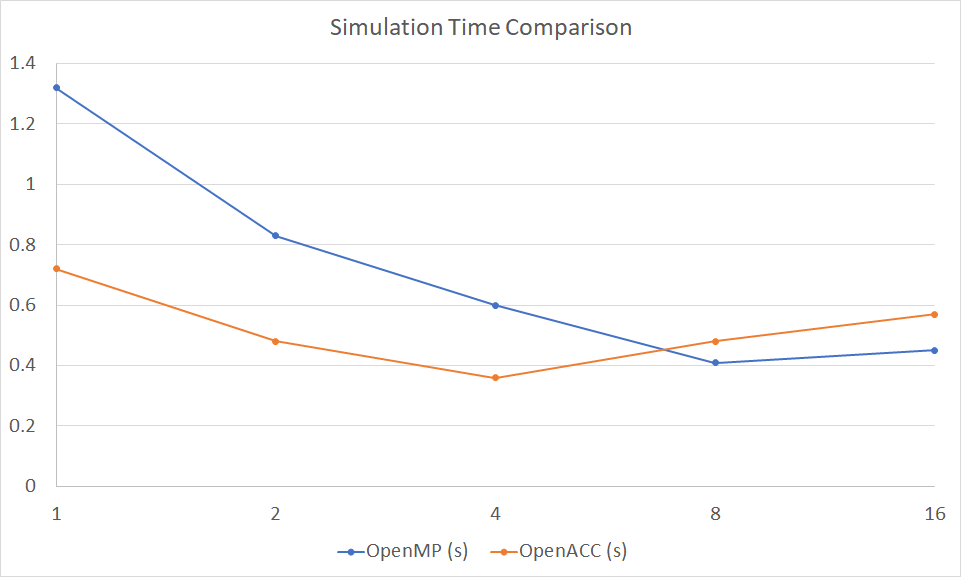
\includegraphics[width=\textwidth]{graph}\\

For discussion, see Section 3. It seems that task switching is more noticeable
for OpenACC (it leads to a decrease in speed even when only using 8 threads).

I also ran the serial code, which took 0.96 seconds to run. So when using 1
thread only, the serial code is actually faster than OpenMP code. This makes
sense because we are doing extra steps for parallelization, like generating and
storing the random numbers first. When using multiple threads, OpenACC looks
like the best choice (but we must be careful about the number of used threads),
closely followed by OpenMP.

\section{Additional Remarks}

Please see the code comments for remarks. I also used git commits to show my
progress!

\end{document}
